\begin{frame}{}
    \LARGE Contrastive Learning: \textbf{Distillation with No Labels (DINO)}
\end{frame}


\begin{frame}[allowframebreaks]{DINO (Distillation with No Labels)}
\begin{figure}
    \centering
    \includegraphics[width=\linewidth,height=0.9\textheight,keepaspectratio]{images/contrastive/slide_86_1_img.jpg}
\end{figure}

\framebreak

\textbf{Why DINO?}
\begin{itemize}
    \item Learns useful features from images without any labels.
    \item Helps the model understand both the big picture and small details.
    \item Combines the strengths of contrastive learning and clustering methods.
\end{itemize}

\framebreak

\begin{columns}[b]
    \column{0.5\textwidth}
        \begin{figure}
            \centering
            \includegraphics[width=\linewidth,height=0.9\textheight,keepaspectratio]{images/contrastive/slide_87_1_img.jpg}
        \end{figure}
    \column{0.5\textwidth}
        \begin{figure}
            \centering
            \includegraphics[width=\linewidth,height=0.9\textheight,keepaspectratio]{images/contrastive/slide_87_2_img.jpg}
        \end{figure}
\end{columns}

\framebreak

\textbf{How does DINO work?}
\begin{itemize}
    \item \textbf{Student and Teacher Networks:} \\
    There are two networks with the same design. The teacher is just a slowly updated version of the student (using EMA).
    \item \textbf{Multi-crop Strategy:} \\
    The model looks at the same image in different ways—two large views and several small crops—to learn features that work at different scales.
    \item \textbf{No Negatives Needed:} \\
    Instead of comparing with negative samples, DINO uses a cross-entropy loss on soft similarity scores between the student and teacher outputs.
    \item \textbf{Avoiding Collapse:} \\
    To make sure the model doesn't just output the same thing for every image, DINO centers and sharpens the teacher's outputs.
\end{itemize}

\framebreak

\begin{figure}
    \centering
    \includegraphics[width=\linewidth,height=0.9\textheight,keepaspectratio]{images/contrastive/slide_88_1_img.jpg}
\end{figure}

\framebreak

\begin{columns}[b]
    \column{0.5\textwidth}
        \begin{figure}
            \centering
            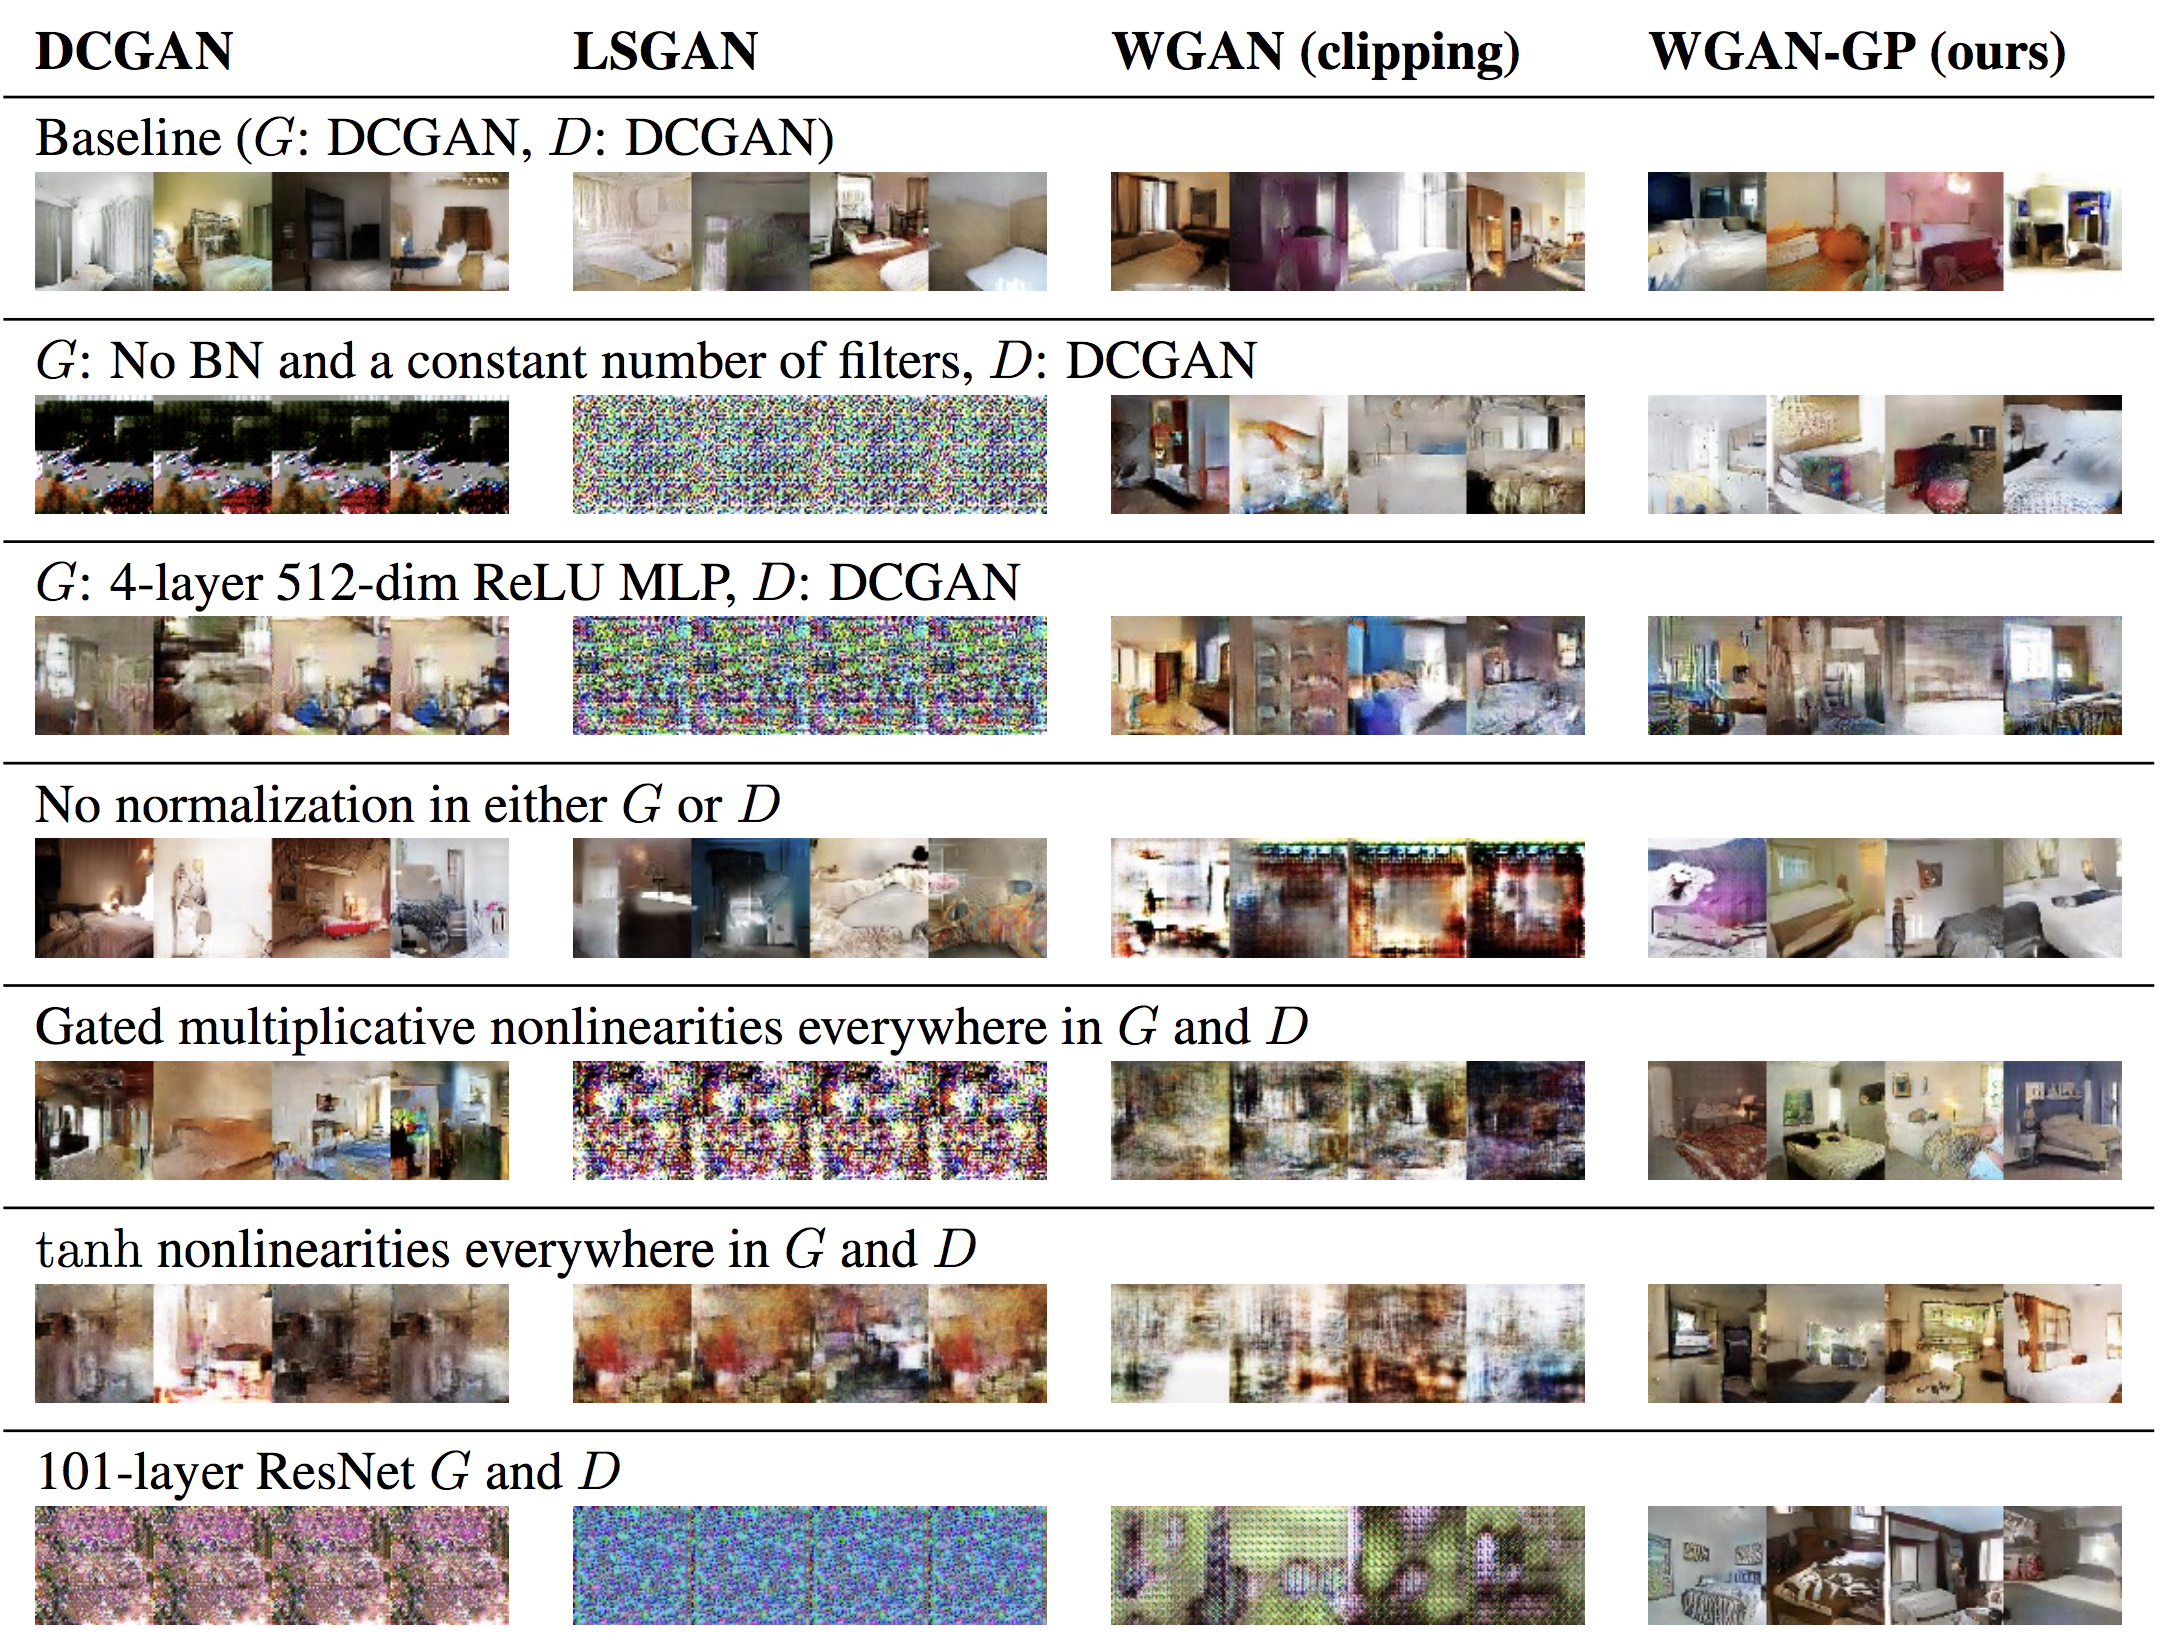
\includegraphics[width=\linewidth,height=0.9\textheight,keepaspectratio]{images/contrastive/slide_89_1_img.png}
        \end{figure}
    \column{0.5\textwidth}
        \begin{figure}
            \centering
            \includegraphics[width=\linewidth,height=0.9\textheight,keepaspectratio]{images/contrastive/slide_89_2_img.png}
        \end{figure}
\end{columns}

\framebreak

\begin{figure}
    \centering
    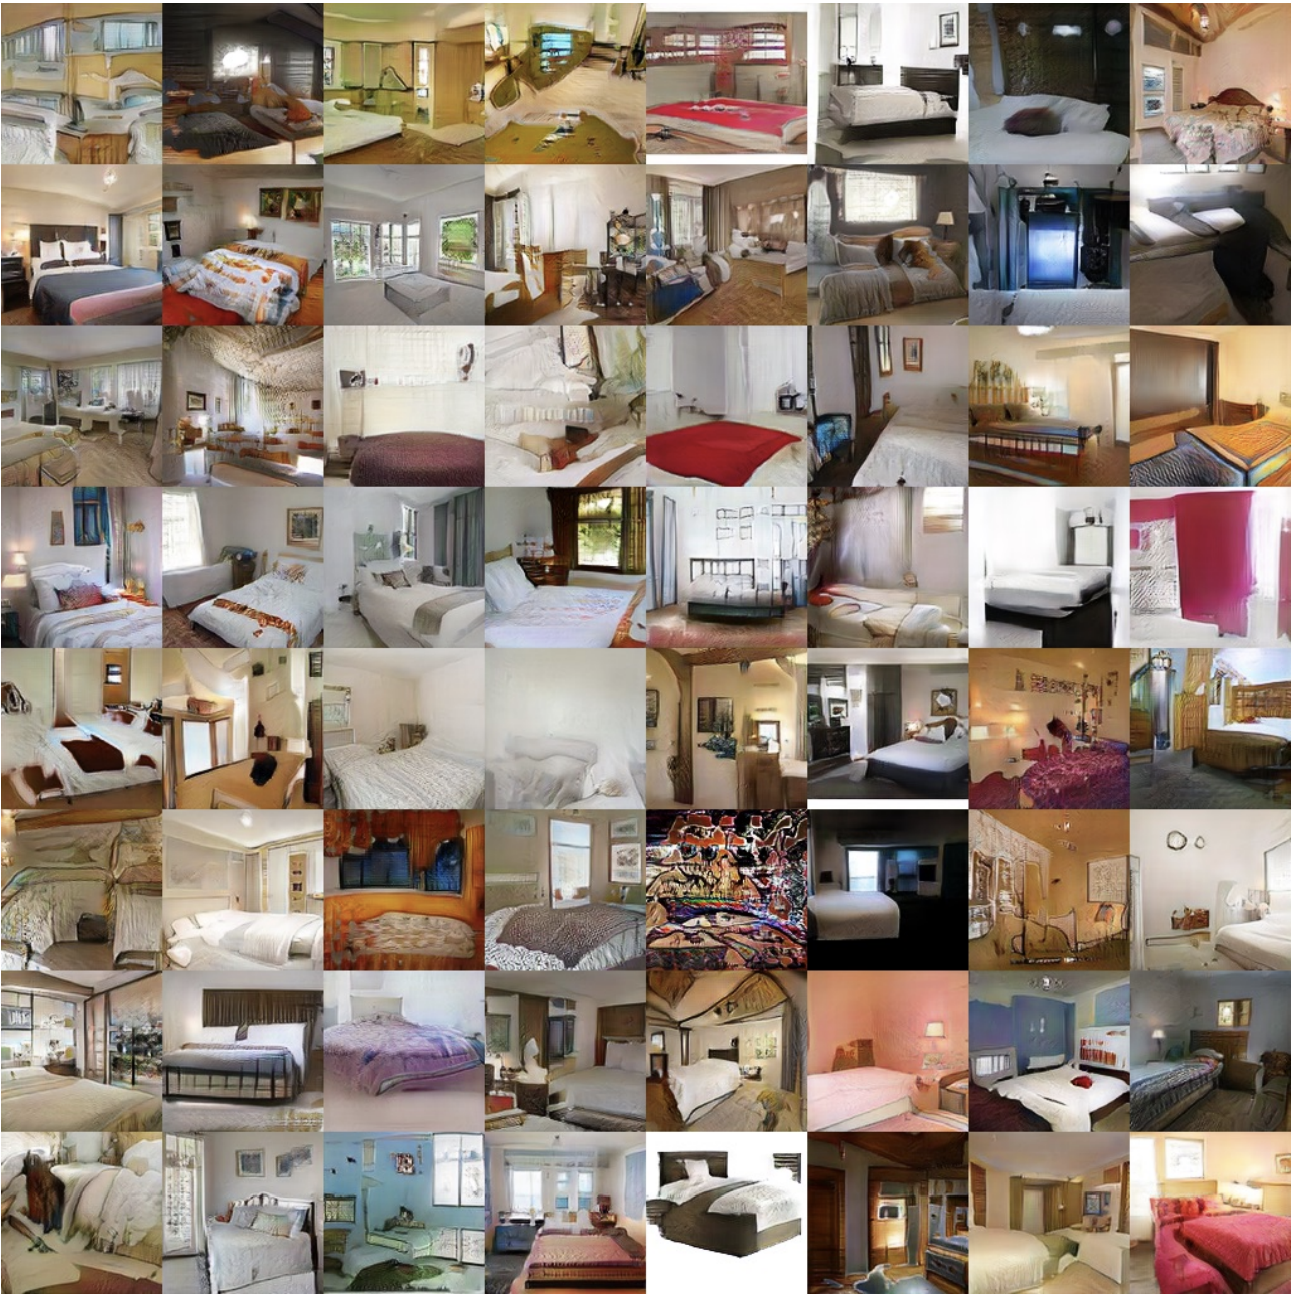
\includegraphics[width=\linewidth,height=0.9\textheight,keepaspectratio]{images/contrastive/slide_90_1_img.jpg}
\end{figure}

\framebreak

\textbf{What makes DINO special?}
\begin{itemize}
    \item Learning from both big and small image parts helps the model understand local details.
    \item Using soft targets (from the teacher) gives the student more useful feedback than just using hard negatives.
\end{itemize}
\end{frame}